% Compile with XeLaTeX (Overleaf: Menu -> Compiler -> XeLaTeX), then BibTeX, then XeLaTeX twice.
\documentclass[11pt]{article}
\usepackage[a4paper,top=2.3cm,bottom=2.4cm,left=2.4cm,right=2.4cm,headsep=0.6cm,headheight=14pt]{geometry}
\usepackage{amsmath,amssymb,amsthm}
\usepackage{mathptmx}
\usepackage[no-math]{fontspec}
\setmainfont{CrimsonPro}[Path=fonts/, Extension=.ttf, Scale=1.12,
  UprightFont=*-Regular, ItalicFont=*-RegularItalic, BoldFont=*-SemiBold, BoldItalicFont=*-SemiBoldItalic]
\setsansfont{OpenSans}[Path=fonts/, Extension=.ttf,
  UprightFont=*-Regular, ItalicFont=*-RegularItalic, BoldFont=*-Bold, BoldItalicFont=*-BoldItalic,
  FontFace={sb}{n}{*-SemiBold}, FontFace={sb}{it}{*-SemiBoldItalic}]
\newcommand{\sbseries}{\fontseries{sb}\selectfont}
\linespread{1.04}
\usepackage{microtype}
\usepackage{xcolor}
\definecolor{navy}{HTML}{1A1A1A}\definecolor{tfred}{HTML}{C8102E}\definecolor{tflred}{HTML}{FBE3E6}
\definecolor{boxgrey}{HTML}{F3F3F3}
\definecolor{linkblue}{HTML}{A50D25}
\definecolor{tfblue}{HTML}{C8102E}\definecolor{tflblue}{HTML}{EDEDED}
\definecolor{tforange}{HTML}{C8102E}\definecolor{tflorange}{HTML}{D9D9D9}
\definecolor{tfaqua}{HTML}{E8737F}\definecolor{tflaqua}{HTML}{FBE3E6}
\definecolor{tfgrey}{HTML}{333333}\definecolor{tflgrey}{HTML}{FFFFFF}
\usepackage{graphicx}
\usepackage[caption=false]{subfig}
\usepackage{booktabs,multirow,array,tabularx}
\usepackage{tikz}
\usetikzlibrary{positioning,arrows.meta,fit,backgrounds,calc,shapes.geometric}
\usepackage{enumitem}
\setlist{leftmargin=*,itemsep=1pt,topsep=3pt}
\usepackage[numbers,sort&compress]{natbib}
\bibpunct[, ]{[}{]}{,}{n}{,}{,}
\setlength{\bibsep}{1.5pt}
\renewcommand{\bibfont}{\sffamily\fontsize{8.8}{11}\selectfont}
\usepackage{caption}
\usepackage{float}
\DeclareCaptionLabelFormat{boldlab}{\textbf{\color{tfred}#1~#2.}}
\captionsetup{font={sf,small}, labelformat=boldlab, labelsep=space, justification=raggedright, singlelinecheck=false, skip=5pt}
\captionsetup[table]{position=top, skip=4pt}
\captionsetup[subfloat]{font={sf,footnotesize}}
\usepackage{titlesec}
\titleformat{\section}{\sffamily\bfseries\Large\color{tfred}}{\thesection.}{0.45em}{}
\titlespacing*{\section}{0pt}{16pt plus 3pt}{6pt}
\titleformat{\subsection}{\sffamily\bfseries\large\color{navy}}{\thesubsection.}{0.45em}{}
\titlespacing*{\subsection}{0pt}{11pt plus 2pt}{4pt}
\titleformat{\subsubsection}{\sffamily\itshape\normalsize\color{navy}}{\thesubsubsection.}{0.45em}{}
\usepackage{fancyhdr}
\pagestyle{fancy}\fancyhf{}
\renewcommand{\headrulewidth}{0.6pt}\renewcommand{\headrule}{{\color{tfred}\hrule height\headrulewidth}}
\fancyhead[L]{\sffamily\footnotesize P.\ KAKAD, A.\ MASAVI AND A.\ MULLA}
\fancyhead[R]{\sffamily\footnotesize IMAGE CAPTIONING ON FLICKR8K\quad\textcolor{tfred}{\textbf{\thepage}}}
\fancypagestyle{first}{\fancyhf{}\renewcommand{\headrulewidth}{0pt}}
\usepackage[colorlinks=true,linkcolor=linkblue,citecolor=linkblue,urlcolor=linkblue]{hyperref}
\setlength{\parindent}{1.3em}
\setlength{\parskip}{0pt}
\setlength{\emergencystretch}{2.5em}\tolerance=1500
\setlength{\tabcolsep}{4.6pt}
\setcounter{topnumber}{3}\setcounter{dbltopnumber}{3}\setcounter{totalnumber}{5}
\renewcommand{\topfraction}{0.9}\renewcommand{\dbltopfraction}{0.9}
\renewcommand{\textfraction}{0.08}\renewcommand{\floatpagefraction}{0.75}\renewcommand{\dblfloatpagefraction}{0.75}
\setlength{\dbltextfloatsep}{12pt plus 2pt minus 2pt}\setlength{\textfloatsep}{10pt plus 2pt minus 2pt}
% table helpers
\newcommand{\tbl}[2]{\caption{#1}{\sffamily\small #2}}
\newcommand{\tabnote}[1]{\par\vspace{3pt}{\noindent\sffamily\footnotesize\raggedright #1\par}}
\newcommand{\best}[1]{\textbf{#1}}
\newcommand{\sd}[1]{{\scriptsize$\,\pm$#1}}
\setlength{\aboverulesep}{1.5pt}\setlength{\belowrulesep}{1.5pt}
\setlength{\heavyrulewidth}{0.7pt}\setlength{\lightrulewidth}{0.4pt}
\usepackage{ragged2e}
\begin{document}
\thispagestyle{first}
{%
\noindent\begin{minipage}[b]{0.62\textwidth}\sffamily\footnotesize\raggedright
DEEP LEARNING COURSE PROJECT REPORT\\
2026, B.TECH CSBS, MPSTME, SVKM'S NMIMS, MUMBAI
\end{minipage}\hfill
\begin{minipage}[b]{0.36\textwidth}\raggedleft\sffamily
\begin{tikzpicture}[baseline]
\foreach \i/\c in {0/tfred,1/navy,2/tfaqua}{\fill[\c] (\i*0.30,0) rectangle ++(0.24,0.24);}
\end{tikzpicture}\ \ {\small\bfseries\color{tfred}Image Captioning Study}\\[1pt]
{\scriptsize\color{tfgrey}Flickr8k\,$\cdot$\,ResNet50\,$\cdot$\,LSTM / GRU\,$\cdot$\,Attention}
\end{minipage}\par\vspace{5pt}
\noindent{\color{tfred}\rule{\textwidth}{1.2pt}}\par\vspace{16pt}
{\sffamily\bfseries\fontsize{19}{24}\selectfont\color{navy}\raggedright
What actually matters in image captioning? A controlled study of encoders, decoders and attention on Flickr8k, with a replication of a hybrid LSTM--GRU model\par}
\vspace{13pt}
{\sffamily\fontsize{11.5}{14}\selectfont Padmanabh Kakad (E025), Abizer Masavi (E034) and Arzaan Mulla (E039)\par}
\vspace{9pt}
{\sffamily\small B.Tech Computer Science and Business Systems, Mukesh Patel School of Technology Management \& Engineering, SVKM's NMIMS, Mumbai, India\par}
\vspace{14pt}
\noindent\begin{minipage}[t]{0.735\textwidth}
{\color{tfred}\vrule width 2.5pt}\colorbox{boxgrey}{\begin{minipage}[t]{\dimexpr\linewidth-2\fboxsep-2.5pt}\vspace{6pt}%
\leftskip=8pt\rightskip=8pt
{\sffamily\bfseries\footnotesize\color{tfred}ABSTRACT}\par\vspace{1pt}
{\sffamily\fontsize{9.4}{12.4}\selectfont\justifying\noindent Image captioning papers often report gains from a new decoder while changing several other things at once, and measure them on a single run with metrics that can be gamed. We ran a controlled study on Flickr8k (6,091 training, 1,000 validation and 1,000 test images) in which exactly one design choice changes at a time, every configuration is trained with three random seeds, and every difference is tested with a paired bootstrap. Part~1 compares three recurrent decoders (LSTM, GRU and the hybrid LSTM$\rightarrow$GRU of Kavitha and Karpagam, 2025) with a frozen or fine-tuned ResNet50 encoder. Part~2 adds soft attention, a Transformer decoder, a CLIP encoder and the pretrained BLIP models as a reference. The encoder matters most: replacing ResNet50 with CLIP raises CIDEr from 0.401 to 0.582 (+45\%). Attention is second (+24\% over the best classic model, CIDEr 0.524). Fine-tuning and the choice of recurrent unit give small but statistically real gains of about 5\%, while the hybrid decoder is no better than a plain GRU ($p=0.40$). Replicating the reference paper's training protocol shows that its reported 0.893 accuracy is largely produced by counting padding tokens: the same kind of model scores 0.79 with padding counted and 0.41 without, at identical caption quality. A reference-free evaluation with CLIPScore agrees with BLEU-4 on the ranking of models trained on the same data (Spearman $\rho=0.92$) but not for a model that writes in a different style. All code, an interactive dashboard with live captioning and per-word attention maps, and the full results are released.\par}\vspace{8pt}
\end{minipage}}
\end{minipage}\hfill
\begin{minipage}[t]{0.235\textwidth}\sffamily\raggedright\vspace{6pt}
{\bfseries\footnotesize\color{tfred}KEYWORDS}\par\vspace{1pt}
{\fontsize{8.6}{11}\selectfont Image captioning; encoder--decoder; attention; LSTM; GRU; CLIP; reproducibility; evaluation metrics; Flickr8k\par}
\vspace{9pt}
{\bfseries\footnotesize\color{tfred}HEADLINE RESULTS}\par\vspace{2pt}
{\fontsize{8.2}{10.6}\selectfont
\textcolor{tfred}{\bfseries +45\%} CIDEr from a CLIP encoder\\
\textcolor{tfred}{\bfseries +24\%} CIDEr from attention\\
\textcolor{tfred}{\bfseries 0.79 $\rightarrow$ 0.41} accuracy once padding is ignored\\
\textcolor{tfgrey}{\bfseries no gain} from the hybrid LSTM--GRU over a plain GRU\par}
\end{minipage}
\vspace{18pt}
}
%=====================================================================
\section{Introduction}

Image captioning asks a model to look at a photograph and write a sentence that describes it, such as \textit{``a brown dog is running through a grassy field''}. The task joins computer vision and language generation, and has become a standard testbed for both. Since the encoder--decoder model of Vinyals et al.\ \cite{vinyals2015}, in which a convolutional network (CNN) encodes the image and a recurrent network (RNN) writes the caption, a large number of variants have been proposed: different CNNs, different recurrent units, stacked and bidirectional decoders, attention over image regions \cite{xu2015,anderson2018}, and Transformer decoders \cite{vaswani2017}.

Comparing these variants is harder than it looks. A typical paper changes the encoder, the decoder, the training recipe and the decoding strategy together, reports a single training run, and measures quality with metrics whose definitions are easy to bend. This project started from one such paper, Kavitha and Karpagam \cite{kavitha2025}, which reports that a ResNet50 encoder with a hybrid LSTM--GRU decoder and beam search reaches an accuracy of 0.8932 and a BLEU-1 score of 0.6034 on Flickr8k. When we began to reproduce it, the first model we trained reached a token accuracy of about 0.44, which raised the question of what the paper's accuracy actually measures, and more broadly of which design choices in a captioning system really matter.

We answer that question with a controlled study. Every configuration shares the same data split, vocabulary, training procedure and evaluation code; exactly one design choice changes between compared configurations; each configuration is trained with three random seeds; and every claimed difference is tested for statistical significance. Our contributions are:

\begin{enumerate}
\item \textbf{A controlled ablation} of three recurrent decoders (LSTM, GRU, hybrid LSTM$\rightarrow$GRU) crossed with a frozen or fine-tuned ResNet50 encoder: six configurations, 18 trained models.
\item \textbf{A replication of the reference paper's protocol} that explains most of its reported accuracy (the ``accuracy illusion'') and clarifies how its BLEU score was computed.
\item \textbf{An extension beyond the classic models}: soft attention, a Transformer decoder, a CLIP image encoder and the pretrained BLIP models, which places the classic results on a scale from a 2015 design to a 2022 model.
\item \textbf{A broader evaluation}: corpus BLEU, METEOR, ROUGE-L and CIDEr; the reference-free CLIPScore; object hallucination; caption diversity; and paired-bootstrap significance tests with Holm correction for every comparison.
\item \textbf{Interpretability and tooling}: per-word attention and Grad-CAM heatmaps, beam-search trees, a t-SNE map of the image features, and an interactive dashboard that captions uploaded or webcam photos live.
\end{enumerate}

Section~\ref{sec:related} reviews related work and the two reference papers. Sections~\ref{sec:data} and~\ref{sec:method} describe the data and models, Section~\ref{sec:setup} the experimental protocol, and Section~\ref{sec:results} the results. Section~\ref{sec:discussion} discusses what they mean, and Section~\ref{sec:conclusion} concludes.

%=====================================================================
\section{Related work}\label{sec:related}

\subsection{Encoder--decoder captioning}
Vinyals et al.\ \cite{vinyals2015} encoded an image with a CNN and used the resulting vector to start an LSTM \cite{hochreiter1997} that generates the caption word by word (``Show and Tell''). Karpathy and Fei-Fei \cite{karpathy2015} aligned image regions with sentence fragments. The gated recurrent unit (GRU) \cite{cho2014} is a lighter alternative to the LSTM with one state vector instead of two. Encoders have followed progress in image classification, from VGG \cite{simonyan2015} to residual networks \cite{he2016}.

\subsection{Attention and Transformers}
A single image vector forces the decoder to describe every part of the image from the same summary. Xu et al.\ \cite{xu2015} let the decoder attend to a grid of image regions and choose different regions for different words (``Show, Attend and Tell''). Luong et al.\ \cite{luong2015} proposed simpler multiplicative attention computed from the decoder's output. Bottom-up attention over detected objects \cite{anderson2018} and Transformer decoders \cite{vaswani2017} followed. More recently, encoders trained on hundreds of millions of image--text pairs, such as CLIP \cite{radford2021}, and pretrained captioners, such as BLIP \cite{li2022blip}, have shifted the field towards large-scale pretraining \cite{mokady2021}.

\subsection{Evaluation}
Captioning is usually evaluated by comparing generated captions with human references using BLEU \cite{papineni2002}, METEOR \cite{banerjee2005}, ROUGE-L \cite{lin2004rouge} and CIDEr \cite{vedantam2015}. These metrics reward overlap with the reference wording, not correctness as such. CLIPScore \cite{hessel2021} instead measures how well a caption matches the image itself using a pretrained image--text model. Object hallucination, captions that mention objects not present in the image, is measured by CHAIR \cite{rohrbach2018}. Differences between systems are commonly tested with paired bootstrap resampling \cite{koehn2004,dror2018}.

\subsection{The two reference papers}
\textbf{Kavitha and Karpagam (2025)} \cite{kavitha2025} compare four CNN encoders with an LSTM decoder on Flickr8k and select ResNet50, then compare seven decoders and propose a hybrid in which an LSTM layer feeds a GRU layer, decoded with beam search. They train for 40 epochs with batch size 32 and Adam at a learning rate of 0.001, and use 1,000 images each for validation and testing. They report an accuracy of 0.8932 for the hybrid model (0.8459 for ResNet50+LSTM and 0.8594 for ResNet50+GRU), and a ``maximum BLEU-1'' of 0.6034 with beam search (0.5142 greedy), computed ``on 40 example images''. The paper does not state how the 40 images were chosen or how the maximum was taken, and its preprocessing section describes band-pass filtering and short-time Fourier transforms of audio signals, which do not apply to images.

\textbf{Ahmad et al.\ (2023)} \cite{ahmad2023} use a CNN encoder and a GRU decoder on MS COCO \cite{lin2014coco}, together with semantic attribute vectors \cite{yao2017} and a module that reconstructs the image's semantic representation from the decoder states. Because they use a different dataset and additional inputs, we cite their numbers for context only.

\textbf{Gap.} Neither paper isolates a single design choice under identical conditions, reports variation across training runs, or tests whether differences are statistically real. Neither evaluates hallucination or uses a reference-free metric.

%=====================================================================
\section{Data}\label{sec:data}

We use Flickr8k \cite{hodosh2013}: 8,091 photographs from Flickr, mostly of people and animals in everyday outdoor scenes, each with five independent human captions (40,455 captions in total). We split by \emph{image}, not by caption, so that all five captions of a photo fall in the same split, and verify automatically that no image appears in two splits. Following the reference paper, 1,000 images are used for validation and 1,000 for testing, leaving 6,091 for training (Table~\ref{tab:data}).

Captions are lower-cased and stripped of punctuation and digits. The vocabulary contains the 2,584 words that occur at least five times in the training captions, plus four special tokens (\texttt{<pad>}, \texttt{<start>}, \texttt{<end>}, \texttt{<unk>}), for 2,588 tokens. Every caption is wrapped in \texttt{<start>} and \texttt{<end>} and padded to 34 tokens.

\begin{table}[tbp]\centering
\tbl{Data split. The split is by image, with a fixed random seed.}
{\begin{tabular}{@{}lrrp{3.2cm}@{}}\toprule
Split & Images & Captions & Use \\\midrule
Training & 6,091 & 30,455 & model weights \\
Validation & 1,000 & 5,000 & early stopping, model selection \\
Test & 1,000 & 5,000 & all reported results \\\bottomrule
\end{tabular}}
\label{tab:data}
\end{table}

%=====================================================================
\section{Models}\label{sec:method}

All models follow the encoder--decoder pattern of Figure~\ref{fig:arch}. The encoder turns a $224\times224$ image into either one vector or a grid of region vectors; the decoder reads the caption so far and predicts the next word.

\begin{figure}[tbp]
\centering
\resizebox{\textwidth}{!}{\begin{tikzpicture}[font=\sffamily\scriptsize, >={Stealth[length=1.8mm]},
  box/.style={draw=tfgrey, rounded corners=2pt, align=center, text width=17mm, minimum height=9mm, inner sep=2pt, line width=0.45pt},
  enc/.style={box, fill=tflblue}, cls/.style={box, fill=tflgrey}, att/.style={box, fill=tflaqua}, alt/.style={box, fill=tflorange}]
\node[enc] (r14) at (0,0) {ResNet50\\stages 1--4\\(frozen)};
\node[enc] (c5) at (2.2,0) {conv5 block\\frozen \textit{or}\\fine-tuned};
\node[enc] (pool) at (4.35,0.95) {avg.\ pool\\2048-d $\mathbf{v}$};
\node[enc] (grid) at (4.35,-0.95) {$7{\times}7$ map\\49 regions};
\node[cls] (bridge) at (6.45,0.95) {bridge\\Dense 256};
\node[att] (proj) at (6.45,-0.95) {Dense 256 +\\LayerNorm};
\node[cls, text width=29mm] (dec) at (9.05,0.95) {\textbf{Classic decoder}\\LSTM / GRU / Hybrid};
\node[att, text width=29mm] (adec) at (9.05,-0.95) {\textbf{Attention decoder}\\LSTM + attention\\or Transformer};
\node[box, text width=19mm] (out) at (11.85,0) {softmax over\\2,588 words};
\node[alt, text width=22mm] (altv) at (4.35,2.25) {VGG16 or CLIP\\512-d vector};
\node[align=center] (img) at (0,1.5) {image\\$224{\times}224{\times}3$};
\draw[->] (img) -- (r14);
\draw[->] (r14) -- (c5);
\draw[->] (c5.east) -- ++(2.5mm,0) |- (pool.west);
\draw[->] (c5.east) -- ++(2.5mm,0) |- (grid.west);
\draw[->] (pool) -- (bridge);
\draw[->] (grid) -- (proj);
\draw[->, dashed, tforange] (altv.east) -| (bridge.north);
\draw[->] (bridge) -- (dec);
\draw[->] (proj) -- (adec);
\draw[->] (dec.east) -- ++(2.5mm,0) |- (out.west);
\draw[->] (adec.east) -- ++(2.5mm,0) |- (out.west);
\end{tikzpicture}}
\caption{Model overview. Classic decoders (Part~1, white boxes) start from the pooled image vector; attention decoders (Part~2, pink boxes) read all 49 regions of ResNet50's final $7\times7$ feature map. In the encoder comparison (dark grey box, red dashed arrow) the pooled ResNet50 vector is replaced by a VGG16 or CLIP vector. The bridge output is the classic decoders' initial state; attention decoders query the projected regions at every word. Each decoder reads the caption so far and predicts the next word.}
\label{fig:arch}
\end{figure}

\subsection{Encoders}
\textbf{Frozen ResNet50.} ResNet50 \cite{he2016} with ImageNet weights is run once over every image, and the global-average-pooled 2,048-dimensional vector $\mathbf{v}$ is stored. A small dense \emph{bridge} layer (256 units) turns this vector into the starting state of the decoder.

\textbf{Fine-tuned ResNet50.} We precompute the output of ResNet50's fourth stage ($14\times14\times1024$) and train the final block (conv5, about 15 million weights) together with the decoder. Batch-normalisation statistics stay frozen. Fine-tuning is done in two stages: each fine-tuned model starts from the trained frozen model of the same seed and continues at a learning rate of $10^{-5}$. (We found that the original project code labelled a configuration ``fine-tuned'' while reusing frozen features; the version reported here updates the conv5 weights.)

\textbf{Region grid (attention models).} The final $7\times7\times2048$ map is reshaped into 49 region vectors, projected to 256 dimensions and layer-normalised. Without normalisation the raw ResNet50 values saturated the attention softmax and the decoder could barely learn (validation loss 2.97 versus 0.87 after four epochs in a small test).

\textbf{VGG16 and CLIP.} For the encoder comparison the pooled ResNet50 vector is replaced by the 512-dimensional pooled VGG16 \cite{simonyan2015} vector or the 512-dimensional CLIP ViT-B/32 image embedding \cite{radford2021}. Everything else is identical to the frozen hybrid configuration.

\subsection{Classic decoders}
Each word is first turned into a vector of 256 numbers (an \emph{embedding}). The decoder then reads the caption one word at a time and, after each word, guesses the next one. The image enters only once, as the decoder's starting state. The three decoders differ only in the recurrent unit:
\begin{itemize}
\item \textbf{LSTM} \cite{hochreiter1997}: keeps two memories (a short-term state and a long-term cell) controlled by three gates.
\item \textbf{GRU} \cite{cho2014}: a simpler unit with one memory and two gates, so it has fewer weights.
\item \textbf{Hybrid LSTM$\rightarrow$GRU} \cite{kavitha2025}: an LSTM layer whose output is passed through a GRU layer.
\end{itemize}
In all three, a final softmax layer turns the decoder's output into a probability for each of the 2,588 words in the vocabulary:
\begin{equation}
P(\text{next word}) = \mathrm{softmax}(W \cdot \text{decoder output}).
\end{equation}
All three use 256 hidden units and differ only in the recurrent part, so the comparison isolates the recurrent unit.

\subsection{Attention decoders}
\textbf{A1: LSTM with soft attention.} Instead of one summary vector, this model sees the photo as 49 regions (a $7\times7$ grid). Before writing each word it:
\begin{enumerate}
\item gives each region a score for how useful it is for the next word,
\item turns the scores into 49 weights that add up to 1 (with a softmax),
\item builds a \emph{context} vector as the weighted average of the regions,
\begin{equation}
\text{context} = w_1\,r_1 + w_2\,r_2 + \dots + w_{49}\,r_{49},
\end{equation}
\item and predicts the next word from its own state together with this context.
\end{enumerate}
The 49 weights form a $7\times7$ map for every word, which we draw as a heatmap (Figure~\ref{fig:heat}). With 2.71 million weights, A1 is the same size as the classic hybrid (2.77 million), so any gain comes from attention, not from a bigger model.

\textbf{A2: Transformer decoder.} The Transformer \cite{vaswani2017} replaces the recurrent unit with attention everywhere: each word looks at the earlier words of the caption and at the 49 image regions. We use three blocks with four attention heads and width 256. Its image attention also gives a map for each word.

\subsection{Training objective}
During training the model sees the correct caption and must predict each next word (\emph{teacher forcing}). The loss is the usual cross-entropy: the more probability the model gives to the correct next word, the lower the loss. Because captions are padded to 34 tokens, we ignore the padding positions and average only over real words:
\begin{equation}
\text{Loss} = -\,\frac{1}{N}\sum_{\text{real words}} \log P(\text{correct next word}),
\end{equation}
where $N$ is the number of real (non-padding) words. The \emph{paper-protocol} replication instead counts the padding positions too, as an unmasked Keras loss does. This small detail turns out to matter a lot (Section~\ref{sec:illusion}).

\subsection{Decoding}
\textbf{Greedy} decoding picks the most probable word at every step. \textbf{Beam search} with width $k$ keeps the $k$ most likely partial captions at every step instead of just one, and at the end returns the most likely complete caption (Figure~\ref{fig:beam} shows an example). Our implementation is batched over images and never generates \texttt{<pad>} or \texttt{<start>} mid-caption.

%=====================================================================
\section{Experimental setup}\label{sec:setup}

\subsection{Configurations}
Table~\ref{tab:configs} lists every configuration. Part~1 is the core ablation; Part~2 goes beyond the course syllabus and is reported separately so that the in-syllabus results stand on their own.

\begin{table}[tbp]\centering
\tbl{Configurations. All classic and attention models use embedding and hidden size 256. ``ft'' = fine-tuned conv5 block.}
{\begin{tabular}{llllrc}\toprule
ID & Encoder & Decoder & Image input & Weights (M) & Seeds\\\midrule
\multicolumn{6}{l}{\textit{Part 1: classic decoders}}\\
C1 & ResNet50, frozen & LSTM & pooled 2048 & 2.38 & 3\\
C2 & ResNet50, frozen & GRU & pooled 2048 & 2.25 & 3\\
C3 & ResNet50, frozen & Hybrid LSTM$\rightarrow$GRU & pooled 2048 & 2.77 & 3\\
C4 & ResNet50, ft & LSTM & stage-4 map & 17.33 & 3\\
C5 & ResNet50, ft & GRU & stage-4 map & 17.20 & 3\\
C6 & ResNet50, ft & Hybrid LSTM$\rightarrow$GRU & stage-4 map & 17.73 & 3\\
PP & ResNet50, frozen & Hybrid, paper protocol & pooled 2048 & 2.77 & 1\\\midrule
\multicolumn{6}{l}{\textit{Encoder comparison}}\\
E1 & VGG16, frozen & Hybrid LSTM$\rightarrow$GRU & pooled 512 & 2.38 & 3\\
E2 & CLIP ViT-B/32, frozen & Hybrid LSTM$\rightarrow$GRU & embedding 512 & 2.38 & 3\\\midrule
\multicolumn{6}{l}{\textit{Part 2: attention}}\\
A1 & ResNet50, frozen & LSTM + soft attention & $7{\times}7$ grid & 2.71 & 3\\
A2 & ResNet50, frozen & Transformer (3 blocks) & $7{\times}7$ grid & 5.03 & 3\\\midrule
\multicolumn{6}{l}{\textit{Pretrained reference (no training)}}\\
B1 & \multicolumn{2}{l}{BLIP-base \cite{li2022blip}} & image & -- & --\\
B2 & \multicolumn{2}{l}{BLIP-large \cite{li2022blip}} & image & -- & --\\\bottomrule
\end{tabular}}
\tabnote{Weights are trainable parameters. For C4--C6 they include the 15 M weights of the conv5 block.}
\label{tab:configs}
\end{table}

\subsection{Training}
All models are trained with Adam \cite{kingma2015} on batches of 32 (Transformer: 64), learning rate $10^{-3}$ (Transformer: $3\times10^{-4}$; fine-tuning: $10^{-5}$), gradient clipping at norm 5, for up to 40 epochs (fine-tuning: 10). Training stops when the validation loss has not improved for five epochs (fine-tuning: three), and the weights of the best epoch are kept. The paper-protocol run (PP) instead follows \cite{kavitha2025} exactly: 40 epochs, batch 32, learning rate 0.001, padding counted in the loss, no early stopping. Every configuration is trained with seeds 1, 2 and 3. Training ran on an NVIDIA L4 GPU (Google Colab): one epoch of a classic model took 7--8\,s, one Transformer epoch about 28\,s, and the nine frozen runs, including evaluation, took 45 minutes in total.

\subsection{Metrics}
All caption metrics are computed on the 1,000 test images against their five references with the official COCO caption evaluation code: corpus BLEU-1 to BLEU-4 \cite{papineni2002}, METEOR 1.5 \cite{banerjee2005}, ROUGE-L \cite{lin2004rouge} and CIDEr \cite{vedantam2015}. In addition:
\begin{itemize}
\item \textbf{Token accuracy}, reported two ways: \emph{masked} (real words only) and \emph{unmasked} (every position, padding included), plus top-5 next-word accuracy.
\item \textbf{CLIPScore} \cite{hessel2021}: CLIP (ViT-L/14) turns the caption and the photo into vectors, and the score is 2.5 times their cosine similarity (how closely they point in the same direction). It needs no human captions. We deliberately use a larger CLIP than the ViT-B/32 used as encoder in E2, so that model is not judged by the network it was built on.
\item \textbf{Object hallucination} (CHAIR-s) \cite{rohrbach2018}: the share of captions that name at least one of 35 object groups (dog, ball, bench, water, \ldots) that none of the five references mention. All person words count as one group, so ``man'' for ``person'' is not counted as hallucination.
\item \textbf{Key-object recall}: the share of images whose caption names the main subject mentioned by at least three of the five references.
\item \textbf{Diversity}: the share of test images that receive a caption no other image receives.
\end{itemize}

\begin{table}[tbp]\centering
\tbl{The evaluation measures in plain words. All scores are between 0 and 1 (CIDEr can exceed 1); higher is better except for hallucination.}
{\begin{tabularx}{\textwidth}{@{}>{\bfseries}lX@{}}\toprule
Measure & What it checks\\\midrule
BLEU-1 / BLEU-4 & How many single words (BLEU-1) or 4-word phrases (BLEU-4) of the caption also appear in the five human captions.\\
METEOR & Like BLEU, but also accepts synonyms and different word forms (``run''/``running'').\\
ROUGE-L & The longest run of words the caption shares, in order, with a human caption.\\
CIDEr & Word overlap that gives more credit to informative words (``frisbee'') than to common ones (``a'', ``the''). Our main measure.\\
CLIPScore & How well the caption matches the \emph{photo itself}, judged by the CLIP model; no human captions needed.\\
Hallucination & How often the caption names an object that is not in the photo.\\
Token accuracy & How often the next word is guessed exactly right. Easy to inflate if padding is counted.\\\bottomrule
\end{tabularx}}
\label{tab:glossary}
\end{table}

\subsection{Statistical testing}
For each comparison, per-image scores (CIDEr, and CLIPScore separately) are averaged over the three seeds and compared on the same images. We resample the 1,000 test images with replacement 10,000 times \cite{koehn2004,dror2018} to obtain a 95\% confidence interval and a $p$-value for the difference (roughly: the chance of seeing a difference this large if the two models were really equal; below 0.05 we call it real), and correct the eleven $p$-values with Holm's method \cite{holm1979}. Seed-to-seed variation is reported separately as $\pm$ one standard deviation.

%=====================================================================
\section{Results}\label{sec:results}

\subsection{Part 1: decoders and fine-tuning}

\begin{table}[tbp]\centering
\tbl{Part 1 results on the 1,000 test images (beam width 5, mean $\pm$ s.d.\ over three seeds). Best value per column in bold.}
{\begin{tabular}{lcccccc}\toprule
Config & BLEU-1 & BLEU-4 & METEOR & ROUGE-L & CIDEr & Key-object\\\midrule
C1 LSTM & 0.581\sd{.006} & 0.168\sd{.006} & 0.175\sd{.004} & 0.422\sd{.005} & 0.377\sd{.024} & 0.608\\
C2 GRU & 0.580\sd{.008} & 0.172\sd{.001} & 0.179\sd{.002} & 0.426\sd{.004} & 0.395\sd{.006} & 0.620\\
C3 Hybrid & 0.586\sd{.014} & 0.174\sd{.004} & 0.179\sd{.000} & 0.428\sd{.001} & 0.401\sd{.006} & 0.615\\
C4 LSTM ft & 0.585\sd{.007} & 0.172\sd{.004} & 0.179\sd{.002} & 0.427\sd{.006} & 0.392\sd{.015} & 0.616\\
C5 GRU ft & \best{0.590}\sd{.010} & 0.179\sd{.002} & \best{0.183}\sd{.001} & 0.435\sd{.001} & 0.414\sd{.004} & 0.630\\
C6 Hybrid ft & \best{0.590}\sd{.004} & \best{0.184}\sd{.002} & \best{0.183}\sd{.001} & \best{0.437}\sd{.002} & \best{0.423}\sd{.003} & \best{0.637}\\\bottomrule
\end{tabular}}
\label{tab:partA}
\end{table}

\begin{figure}[tbp]
\centering
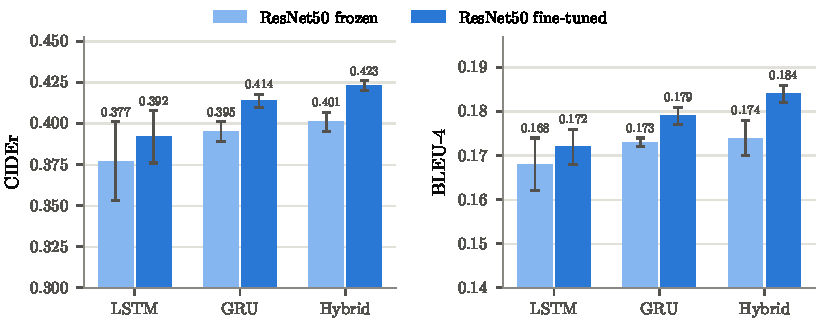
\includegraphics[width=\textwidth]{figures/fig_ablation.pdf}
\caption{Part~1 ablation. Fine-tuning ResNet50's last block raises CIDEr and BLEU-4 for every decoder; the GRU-based decoders lead the LSTM. Error bars: $\pm$ one standard deviation over three seeds.}
\label{fig:ablation}
\end{figure}

Table~\ref{tab:partA} and Figure~\ref{fig:ablation} show the six Part~1 configurations. The differences are small. The best model, C6 (hybrid decoder, fine-tuned encoder), reaches CIDEr 0.423 and BLEU-4 0.184, against 0.377 and 0.168 for the plain LSTM. Fine-tuning helps all three decoders by 0.015--0.022 CIDEr, and both GRU-based decoders beat the LSTM. The C1 LSTM is also the least stable across seeds ($\pm$0.024 CIDEr).

\subsection{Greedy versus beam search}

\begin{figure}[tbp]
\centering
\subfloat[Greedy vs beam search (BLEU-1)]{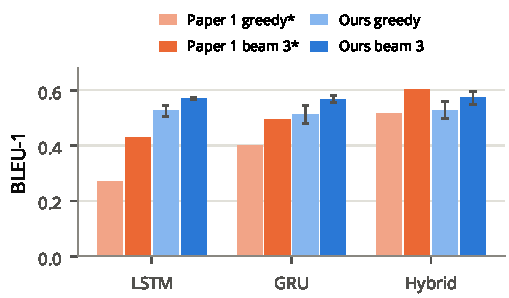
\includegraphics[width=0.48\textwidth]{figures/fig_decoding.pdf}\label{fig:decoding}}\hfill
\subfloat[The accuracy illusion]{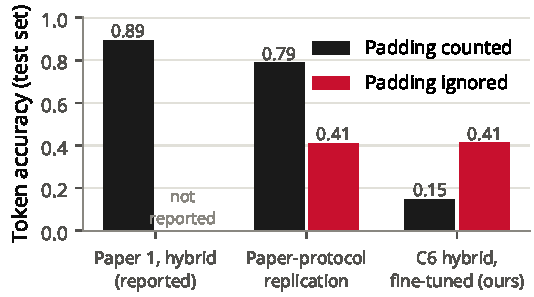
\includegraphics[width=0.48\textwidth]{figures/fig_illusion.pdf}\label{fig:illusion}}
\caption{(a) Beam search adds 0.04--0.06 BLEU-1 for every decoder. *Paper~1 values are its ``maximum BLEU-1 on 40 example images''; ours are corpus BLEU-1 on all 1,000 test images. (b) Token accuracy with and without padding. The paper-protocol replication and C6 write captions of the same quality (BLEU-1 0.588 vs 0.590), yet their padded accuracies differ fivefold.}
\end{figure}

Beam search with $k=3$ improves BLEU-1 for every frozen decoder, by +0.044 (LSTM), +0.056 (GRU) and +0.045 (hybrid) (Figure~\ref{fig:decoding}), which confirms the reference paper's qualitative claim. The large gaps between decoders in the paper (greedy BLEU-1 of 0.27 for the LSTM versus 0.51 for the hybrid) do not reappear: under identical conditions our greedy scores are 0.525, 0.512 and 0.528. On a 40-image sample (the paper's protocol) the hybrid's BLEU-1 is 0.600 $\pm$ 0.016 greedy and 0.596 $\pm$ 0.038 with beam 3, close to the paper's 0.6034 but with a seed-to-seed spread of up to four points, which shows how unreliable a 40-image comparison is.

\subsection{Replication: the accuracy illusion}\label{sec:illusion}

\begin{table}[tbp]\centering
\tbl{The accuracy illusion. Paper-protocol replication (PP) versus our best Part 1 model (C6), both on the 1,000 test images.}
{\begin{tabular}{lccc}\toprule
Measure & Paper 1 \cite{kavitha2025} & PP replication & C6 (ours)\\\midrule
Token accuracy, padding counted & 0.8932 & 0.788 & 0.149\\
Token accuracy, padding ignored & not reported & 0.411 & 0.413\\
Top-5 next-word accuracy & not reported & 0.691 & 0.692\\
BLEU-1, all 1,000 test images & not reported & 0.588 & 0.590\\
BLEU-1, 40-image sample & 0.6034 & 0.579 & 0.591\sd{.010}\\
Best single-image BLEU-1 among 40 & -- & 0.909 & 0.967\sd{.058}\\\bottomrule
\end{tabular}}
\tabnote{The paper's ``maximum BLEU-1 on 40 example images'' is undefined; our 40-image values use the first 40 test images. Reading it as the best single image gives values near 1.}
\label{tab:illusion}
\end{table}

A padded caption of 34 tokens typically contains about a dozen real tokens followed by \texttt{<pad>}. A model trained with padding in the loss learns that \texttt{<pad>} follows \texttt{<end>}, which is trivial, and gains accuracy on every padded position. Table~\ref{tab:illusion} and Figure~\ref{fig:illusion} show the effect. Our replication of the paper's protocol reaches 0.788 token accuracy with padding counted, but only 0.411 on real words, and its captions are no better than C6's, whose padded accuracy is 0.149 because it was never trained to predict padding. Padding therefore explains most of the paper's 0.8932. It does not explain all of it: details the paper does not report, such as the exact maximum length or whether the accuracy is a training figure, could account for the remaining gap. The replication also overfits under the fixed 40-epoch schedule: its validation loss is lowest at epoch 19 and rises afterwards.

\subsection{Encoder comparison}

\begin{figure}[tbp]
\centering
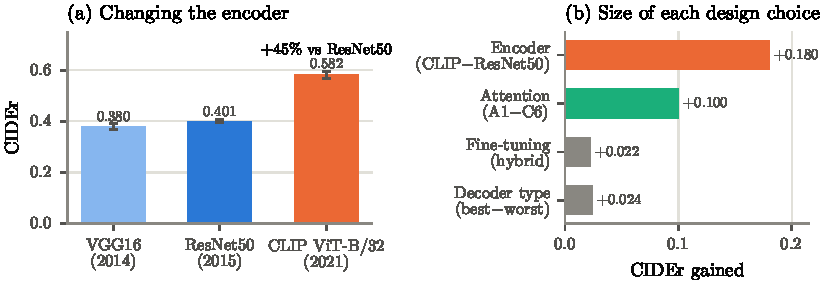
\includegraphics[width=\textwidth]{figures/fig_encoders.pdf}
\caption{(a) Same hybrid decoder, three encoders. (b) CIDEr gained by each design choice, for comparison: the encoder dominates.}
\label{fig:encoders}
\end{figure}

\begin{table}[tbp]\centering
\tbl{Encoder comparison (hybrid decoder, frozen encoder, beam 5, three seeds).}
{\begin{tabular}{llccccc}\toprule
Encoder & Year & BLEU-1 & BLEU-4 & METEOR & CIDEr & Key-object\\\midrule
VGG16 & 2014 & 0.584\sd{.002} & 0.167\sd{.009} & 0.174\sd{.001} & 0.380\sd{.011} & 0.596\\
ResNet50 & 2015 & 0.586\sd{.014} & 0.174\sd{.004} & 0.179\sd{.000} & 0.401\sd{.006} & 0.615\\
CLIP ViT-B/32 & 2021 & \best{0.655}\sd{.004} & \best{0.233}\sd{.006} & \best{0.217}\sd{.001} & \best{0.582}\sd{.014} & \best{0.790}\\\bottomrule
\end{tabular}}
\label{tab:encoders}
\end{table}

Changing only the image features has by far the largest effect in the study (Table~\ref{tab:encoders}, Figure~\ref{fig:encoders}). ResNet50 beats VGG16 by 0.021 CIDEr, consistent with the reference paper's choice of ResNet50, though by a small margin. CLIP's embedding, learned from image--text pairs, raises CIDEr by 0.180 (+45\%) and key-object recall from 62\% to 79\%, with a decoder that has not changed and is smaller than with ResNet50 features. The spread across all three recurrent decoders is only 0.024 CIDEr.

\subsection{Part 2: attention and the pretrained ceiling}

\begin{table}[tbp]\centering
\tbl{Part 2: attention models, the CLIP encoder and the pretrained reference (beam 5; BLIP beam 3).}
{\begin{tabular}{lcccccc}\toprule
Model & BLEU-1 & BLEU-4 & METEOR & CIDEr & Key-object & Unique\\\midrule
C6 Hybrid ft (best Part 1) & 0.590 & 0.184 & 0.183 & 0.423 & 0.637 & 38.8\%\\
A1 LSTM + attention & 0.629\sd{.002} & 0.221\sd{.005} & 0.203\sd{.001} & 0.524\sd{.008} & 0.657 & 84.7\%\\
A2 Transformer & 0.617\sd{.010} & 0.210\sd{.005} & 0.199\sd{.004} & 0.500\sd{.007} & 0.641 & 88.0\%\\
E2 Hybrid + CLIP & 0.655\sd{.004} & 0.233\sd{.006} & 0.217\sd{.001} & 0.582\sd{.014} & 0.790 & --\\\midrule
B1 BLIP-base & 0.648 & 0.263 & 0.212 & 0.665 & 0.716 & 79.0\%\\
B2 BLIP-large & 0.626 & 0.206 & 0.259 & 0.693 & 0.841 & 91.3\%\\\bottomrule
\end{tabular}}
\tabnote{``Unique'' is the share of test images whose caption no other image receives. BLIP was pretrained on about 129 million web images and is a reference point, not a like-for-like competitor.}
\label{tab:partB}
\end{table}

\begin{figure}[tbp]
\centering
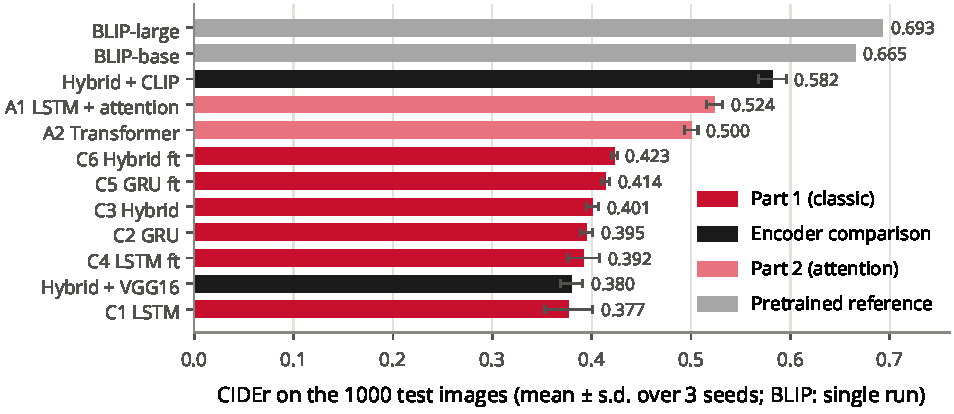
\includegraphics[width=\textwidth]{figures/fig_all_models.pdf}
\caption{CIDEr for every model on the 1,000 test images.}
\label{fig:all}
\end{figure}

Attention is the second-largest effect (Table~\ref{tab:partB}, Figure~\ref{fig:all}). With the same frozen ResNet50 and the same number of weights as the classic hybrid, the attention LSTM (A1) raises CIDEr from 0.423 to 0.524 (+24\%) and BLEU-4 from 0.184 to 0.221. The Transformer (A2) is slightly behind A1 on CIDEr (0.500): with 6,091 training images it overfits quickly (best epoch 6 for one seed, with training accuracy 0.54 against 0.40 on validation). Attention also changes how the models behave. Only 38.8\% of C6's test captions are unique, because it often falls back on a safe sentence such as ``a dog runs through the grass''; with attention, 85--88\% are unique.

The pretrained BLIP models score highest on CIDEr (0.665 and 0.693). BLIP-large, however, has a lower BLEU-4 (0.206) than our attention LSTM, while naming the main subject far more often (84\% against 66\%). Section~\ref{sec:clipscore} examines this contradiction.

\subsection{Which differences are real?}

\begin{figure}[tbp]
\centering
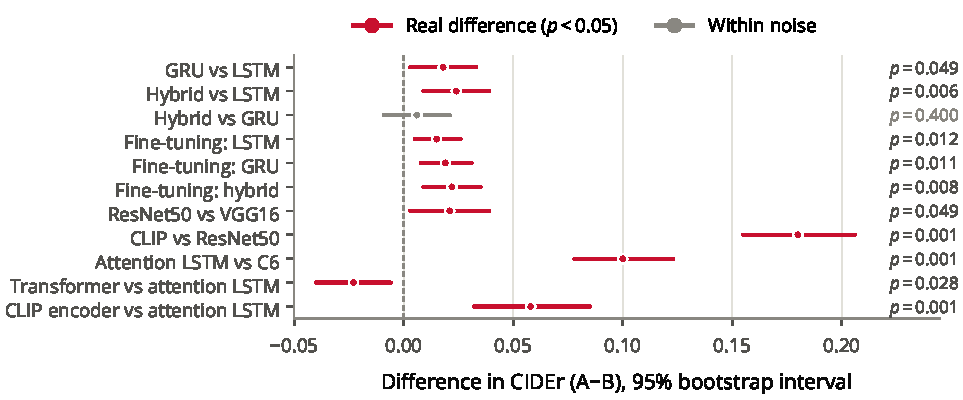
\includegraphics[width=\textwidth]{figures/fig_forest.pdf}
\caption{Paired bootstrap over the 1,000 test images (10,000 resamples, seeds averaged), CIDEr. Red: difference unlikely to be due to which images were sampled (Holm-corrected $p<0.05$).}
\label{fig:forest}
\end{figure}

Figure~\ref{fig:forest} tests every comparison the conclusions rely on. The two large effects, CLIP over ResNet50 (+0.180, 95\% CI [0.155, 0.206]) and attention over the best classic model (+0.100, [0.078, 0.123]), are unambiguous. Fine-tuning helps all three decoders significantly but modestly (+0.015 to +0.022). GRU and the hybrid beat the LSTM, the GRU only borderline ($p=0.049$). \textbf{The hybrid decoder, the central proposal of \cite{kavitha2025}, is not distinguishable from a plain GRU} (+0.006, CI [$-$0.009, 0.021], $p=0.40$), and the CLIPScore test gives the same verdict ($p=0.81$). The Transformer is slightly worse than A1 on CIDEr ($p=0.028$) but equal on CLIPScore ($p=0.51$), so we treat the two attention models as tied.

\subsection{Reference-free evaluation with CLIPScore}\label{sec:clipscore}

\begin{figure}[tbp]
\centering
\subfloat[CLIPScore vs BLEU-4]{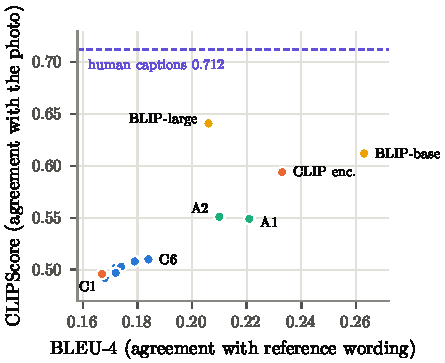
\includegraphics[width=0.56\textwidth]{figures/fig_clipscore.pdf}\label{fig:clipscore}}\hfill
\begin{minipage}[b]{0.40\textwidth}\centering\sffamily\footnotesize\setlength{\tabcolsep}{3.5pt}
\begin{tabular}{lcc}\toprule
Model & CLIP-S & BLEU-4 rank\\\midrule
Human reference & \best{0.712} & --\\
BLIP-large & 0.641 & 5\\
BLIP-base & 0.612 & 1\\
Hybrid + CLIP & 0.594 & 2\\
A2 Transformer & 0.551 & 4\\
A1 LSTM + att. & 0.549 & 3\\
PP replication & 0.514 & 8\\
C6 Hybrid ft & 0.510 & 6\\
C3 Hybrid & 0.503 & 9\\
C1 LSTM & 0.492 & 12\\\bottomrule
\end{tabular}\\[4pt]
{\footnotesize (b) Ranked by CLIPScore}
\end{minipage}
\caption{CLIPScore (CLIP ViT-L/14) judges each caption against the photo, without references. One human reference per image, scored the same way, is the ceiling.}
\end{figure}

BLEU, METEOR and CIDEr reward agreement with the five reference sentences. CLIPScore judges the caption against the image alone. The human reference scores highest (0.712), which shows that the scorer behaves sensibly. Across all twelve models the two metrics largely agree (Spearman $\rho=0.92$ between CLIPScore and BLEU-4): \textbf{for models trained on the same data, BLEU ranks systems correctly}. The exception is BLIP-large, second by CLIPScore but fifth by BLEU-4. Its captions are written in a different style (``there is a man laying on a bench with a dog next to him'') from Flickr8k's short references, and BLEU penalises the wording, not the content. Our best trained model reaches 0.594, still well below human captions.

\subsection{Hallucination and error types}

\begin{figure}[tbp]
\centering
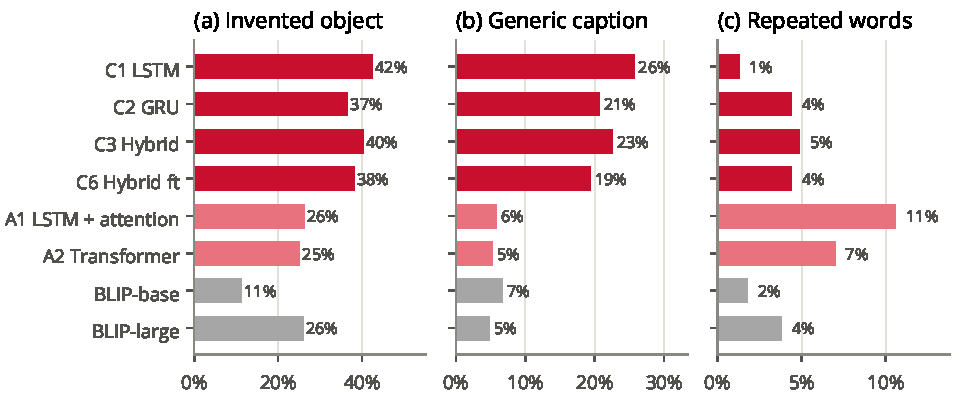
\includegraphics[width=\textwidth]{figures/fig_hallucination.pdf}
\caption{(a) Captions naming an object no reference mentions (CHAIR-s); (b) captions among each model's most frequent, generic sentences; (c) captions that repeat a word or phrase. Error types are detected automatically and are approximate.}
\label{fig:halluc}
\end{figure}

Classic models name an object that is not in the image in 37--43\% of captions; attention cuts this to 25--26\%, and BLIP-base to 11\% (Figure~\ref{fig:halluc}). The most frequent invented objects for classic models are benches, grass and sports equipment, the most common objects in the training captions. Attention also reduces generic captions from about 20\% to 6\%. Its weakness is repetition: 11\% of A1's captions repeat a word or phrase (``a man sitting on a bench on a bench''), against 4\% for C6. About a third of all captions from every Part~1 model name the wrong main subject, typically the wrong kind of person.

\subsection{Qualitative analysis}

\begin{figure}[tbp]
\centering
\subfloat[]{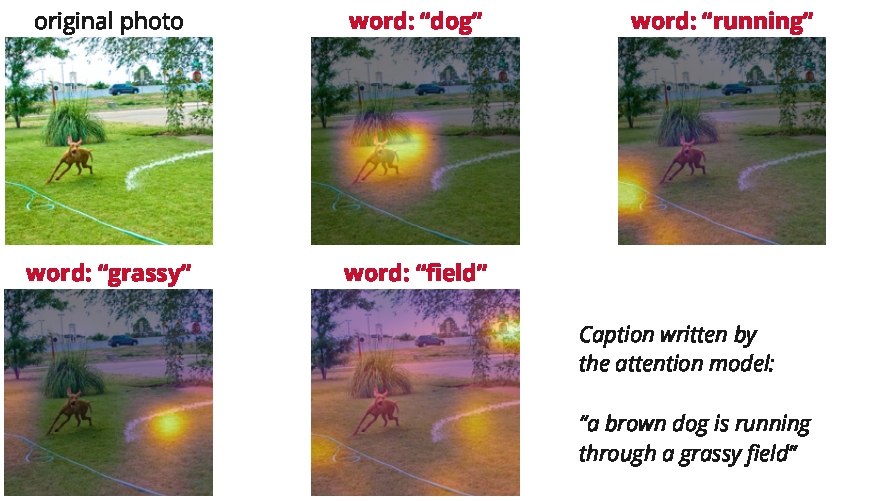
\includegraphics[width=\textwidth]{figures/fig_heatmap_a.pdf}}\\[6pt]
\subfloat[]{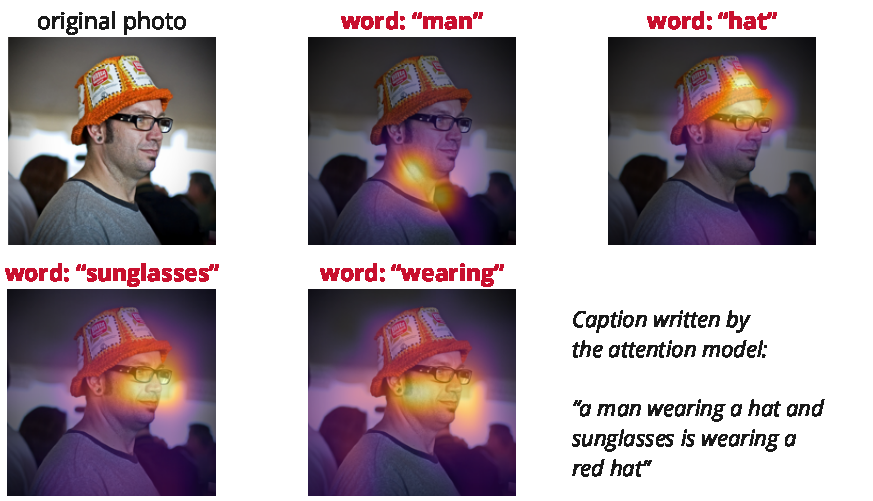
\includegraphics[width=\textwidth]{figures/fig_heatmap_b.pdf}}
\caption{Where the attention model (A1) looks while writing each word. Bright areas got the most attention. (a) It looks at the dog for ``dog'' and at the grass for ``grassy'' and ``field''. (b) It looks at the hat for ``hat'' and at the eyes for ``sunglasses''. Caption (b) also shows A1's habit of repeating itself.}
\label{fig:heat}
\end{figure}

\begin{figure}[tbp]
\centering
\begin{tikzpicture}[font=\sffamily\normalsize, w/.style={draw=black!45, rounded corners=2pt, minimum width=27mm, minimum height=5.6mm, inner sep=1pt, fill=white}, win/.style={w, draw=tfred, fill=tflred, line width=0.8pt, font=\sffamily\normalsize\bfseries}]
\node[font=\sffamily\scriptsize, text=black!55, anchor=east] at (-1.6,0.00) {step 0};
\node[win] (n0_0) at (4.1,0.00) {\textless{}start\textgreater{}};
\node[font=\sffamily\scriptsize, text=black!55, anchor=east] at (-1.6,-1.07) {step 1};
\node[win] (n1_0) at (0,-1.07) {a};
\node[w] (n1_1) at (4.1,-1.07) {the};
\node[w] (n1_2) at (8.2,-1.07) {an};
\node[font=\sffamily\scriptsize, text=black!55, anchor=east] at (-1.6,-2.15) {step 2};
\node[win] (n2_0) at (0,-2.15) {man};
\node[w] (n2_1) at (4.1,-2.15) {woman};
\node[w] (n2_2) at (8.2,-2.15) {man};
\node[font=\sffamily\scriptsize, text=black!55, anchor=east] at (-1.6,-3.22) {step 3};
\node[win] (n3_0) at (0,-3.22) {in};
\node[w] (n3_1) at (4.1,-3.22) {wearing};
\node[w] (n3_2) at (8.2,-3.22) {with};
\node[font=\sffamily\scriptsize, text=black!55, anchor=east] at (-1.6,-4.29) {step 4};
\node[win] (n4_0) at (0,-4.29) {a};
\node[w] (n4_1) at (4.1,-4.29) {a};
\node[w] (n4_2) at (8.2,-4.29) {a};
\node[font=\sffamily\scriptsize, text=black!55, anchor=east] at (-1.6,-5.37) {step 5};
\node[w] (n5_0) at (0,-5.37) {black};
\node[win] (n5_1) at (4.1,-5.37) {blue};
\node[w] (n5_2) at (8.2,-5.37) {red};
\node[font=\sffamily\scriptsize, text=black!55, anchor=east] at (-1.6,-6.44) {step 6};
\node[w] (n6_0) at (0,-6.44) {shirt};
\node[win] (n6_1) at (4.1,-6.44) {shirt};
\node[w] (n6_2) at (8.2,-6.44) {shirt};
\node[font=\sffamily\scriptsize, text=black!55, anchor=east] at (-1.6,-7.50) {step 7};
\node[w] (n7_0) at (0,-7.50) {and};
\node[win] (n7_1) at (4.1,-7.50) {and};
\node[w] (n7_2) at (8.2,-7.50) {and};
\node[font=\sffamily\scriptsize, text=black!55, anchor=east] at (-1.6,-8.57) {step 8};
\node[w] (n8_0) at (0,-8.57) {a};
\node[w] (n8_1) at (4.1,-8.57) {sunglasses};
\node[win] (n8_2) at (8.2,-8.57) {sunglasses};
\node[font=\sffamily\scriptsize, text=black!55, anchor=east] at (-1.6,-9.64) {step 9};
\node[w] (n9_0) at (0,-9.64) {is};
\node[win] (n9_1) at (4.1,-9.64) {is};
\node[w] (n9_2) at (8.2,-9.64) {black};
\node[font=\sffamily\scriptsize, text=black!55, anchor=east] at (-1.6,-10.72) {step 10};
\node[w] (n10_0) at (0,-10.72) {holding};
\node[w] (n10_1) at (4.1,-10.72) {shirt};
\node[win] (n10_2) at (8.2,-10.72) {holding};
\node[font=\sffamily\scriptsize, text=black!55, anchor=east] at (-1.6,-11.79) {step 11};
\node[w] (n11_0) at (0,-11.79) {a};
\node[win] (n11_1) at (4.1,-11.79) {a};
\node[w] (n11_2) at (8.2,-11.79) {is};
\node[font=\sffamily\scriptsize, text=black!55, anchor=east] at (-1.6,-12.86) {step 12};
\node[w] (n12_0) at (0,-12.86) {cup};
\node[win] (n12_1) at (4.1,-12.86) {cup};
\node[w] (n12_2) at (8.2,-12.86) {drink};
\node[font=\sffamily\scriptsize, text=black!55, anchor=east] at (-1.6,-13.93) {step 13};
\node[win] (n13_0) at (0,-13.93) {\textless{}end\textgreater{}};
\node[w] (n13_1) at (4.1,-13.93) {\textless{}end\textgreater{}};
\node[w] (n13_2) at (8.2,-13.93) {\textless{}end\textgreater{}};
\draw[tfred, line width=1.3pt] (n0_0.south) -- (n1_0.north);
\draw[black!55, line width=0.65pt] (n0_0.south) -- (n1_1.north);
\draw[black!55, line width=0.65pt] (n0_0.south) -- (n1_2.north);
\draw[tfred, line width=1.3pt] (n1_0.south) -- (n2_0.north);
\draw[black!55, line width=0.65pt] (n1_0.south) -- (n2_1.north);
\draw[black!55, line width=0.65pt] (n1_1.south) -- (n2_2.north);
\draw[tfred, line width=1.3pt] (n2_0.south) -- (n3_0.north);
\draw[black!55, line width=0.65pt] (n2_0.south) -- (n3_1.north);
\draw[black!55, line width=0.65pt] (n2_0.south) -- (n3_2.north);
\draw[tfred, line width=1.3pt] (n3_0.south) -- (n4_0.north);
\draw[black!55, line width=0.65pt] (n3_1.south) -- (n4_1.north);
\draw[black!55, line width=0.65pt] (n3_2.south) -- (n4_2.north);
\draw[black!55, line width=0.65pt] (n4_0.south) -- (n5_0.north);
\draw[tfred, line width=1.3pt] (n4_0.south) -- (n5_1.north);
\draw[black!55, line width=0.65pt] (n4_0.south) -- (n5_2.north);
\draw[black!55, line width=0.65pt] (n5_0.south) -- (n6_0.north);
\draw[tfred, line width=1.3pt] (n5_1.south) -- (n6_1.north);
\draw[black!55, line width=0.65pt] (n5_2.south) -- (n6_2.north);
\draw[black!55, line width=0.65pt] (n6_0.south) -- (n7_0.north);
\draw[tfred, line width=1.3pt] (n6_1.south) -- (n7_1.north);
\draw[black!55, line width=0.65pt] (n6_2.south) -- (n7_2.north);
\draw[black!55, line width=0.65pt] (n7_0.south) -- (n8_0.north);
\draw[black!55, line width=0.65pt] (n7_0.south) -- (n8_1.north);
\draw[tfred, line width=1.3pt] (n7_1.south) -- (n8_2.north);
\draw[black!55, line width=0.65pt] (n8_1.south) -- (n9_0.north);
\draw[tfred, line width=1.3pt] (n8_2.south) -- (n9_1.north);
\draw[black!55, line width=0.65pt] (n8_0.south) -- (n9_2.north);
\draw[black!55, line width=0.65pt] (n9_0.south) -- (n10_0.north);
\draw[black!55, line width=0.65pt] (n9_2.south) -- (n10_1.north);
\draw[tfred, line width=1.3pt] (n9_1.south) -- (n10_2.north);
\draw[black!55, line width=0.65pt] (n10_0.south) -- (n11_0.north);
\draw[tfred, line width=1.3pt] (n10_2.south) -- (n11_1.north);
\draw[black!55, line width=0.65pt] (n10_1.south) -- (n11_2.north);
\draw[black!55, line width=0.65pt] (n11_0.south) -- (n12_0.north);
\draw[tfred, line width=1.3pt] (n11_1.south) -- (n12_1.north);
\draw[black!55, line width=0.65pt] (n11_0.south) -- (n12_2.north);
\draw[tfred, line width=1.3pt] (n12_1.south) -- (n13_0.north);
\draw[black!55, line width=0.65pt] (n12_0.south) -- (n13_1.north);
\draw[black!55, line width=0.65pt] (n12_2.south) -- (n13_2.north);
\node[font=\sffamily\small\bfseries, text=black!60] at (0,0.69) {beam rank 1};\node[font=\sffamily\small\bfseries, text=black!60] at (4.1,0.69) {beam rank 2};\node[font=\sffamily\small\bfseries, text=black!60] at (8.2,0.69) {beam rank 3};
\end{tikzpicture}
\caption{Beam search in action (C6 model, beam width 3). Each row is one step of writing; at every step the model keeps its three best partial captions. The red path is the final winner: \textit{``a man in a blue shirt and sunglasses is holding a cup''}. Greedy decoding, which only ever keeps the single best word, wrote \textit{``a man in a black shirt and a black shirt is sitting on a \textless unk\textgreater{} chair''}. Beam search escaped because it kept ``blue'' alive at step 5 even though ``black'' looked better at that moment.}
\label{fig:beam}
\end{figure}

\textbf{Attention maps.} Figure~\ref{fig:heat} shows that A1's attention follows the content of each word: object words attend to the object, and scene words to the background. For classic models without attention we computed Grad-CAM \cite{selvaraju2017} exactly from the $7\times7$ grid, since the pooled vector is its average; these maps are available in the dashboard.

\textbf{Beam search.} Figure~\ref{fig:beam} shows beam search escaping the repetition and the unknown word of the greedy path by keeping a lower-probability early choice (``blue'') that leads to a better sentence.

\begin{figure}[tbp]
\centering
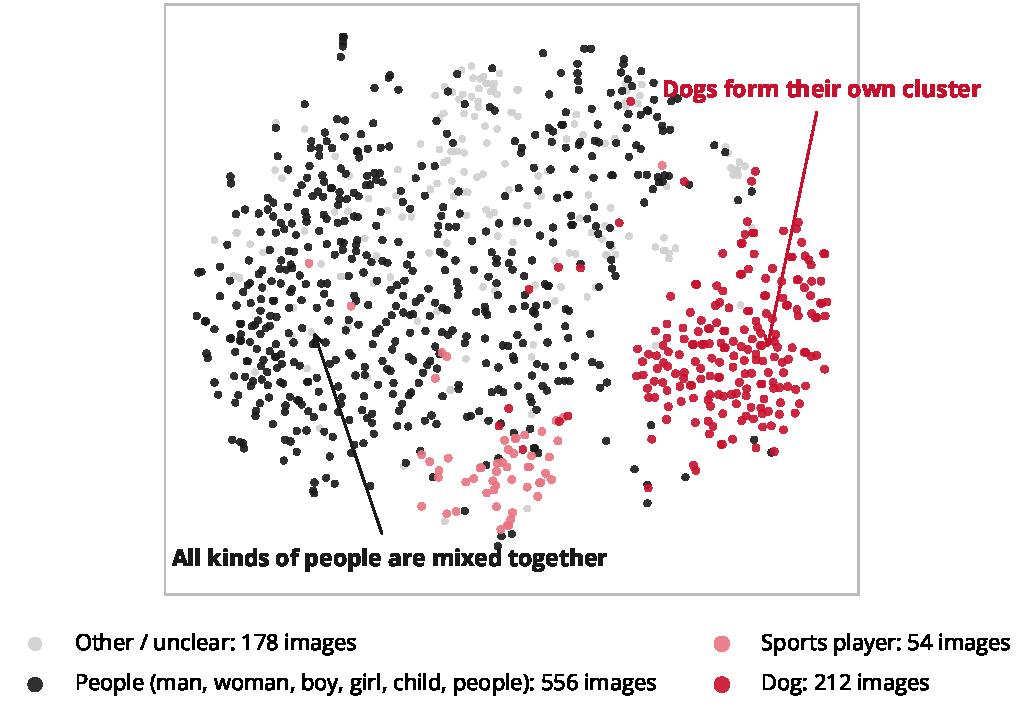
\includegraphics[width=0.92\textwidth]{figures/fig_tsne.pdf}
\caption{A 2-D map of what the encoder ``sees'' (t-SNE of the ResNet50 features of the 1,000 test images). Each dot is one photo; similar-looking photos land close together. Colour is the main subject named in the human captions. Dogs form their own cluster, but the different kinds of people are mixed, which is why the models often name the wrong person. Redrawn from the Colab output with the people categories merged.}
\label{fig:tsne}
\end{figure}

\begin{figure}[tbp]
\centering
\noindent\begin{minipage}[t]{0.315\textwidth}\centering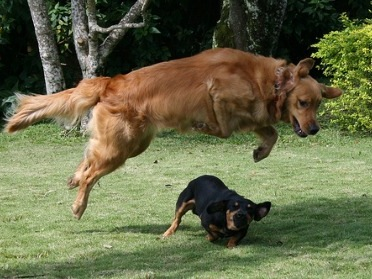
\includegraphics[width=\linewidth]{figures/fail/f00c.jpg}\\[2pt]{\sffamily\footnotesize\raggedright\textit{``two dogs play in the grass''}\\ \textcolor{tfred}{\scriptsize\bfseries INVENTED OBJECT, WRONG COUNT, GENERIC}\par}\end{minipage}\hfill\begin{minipage}[t]{0.315\textwidth}\centering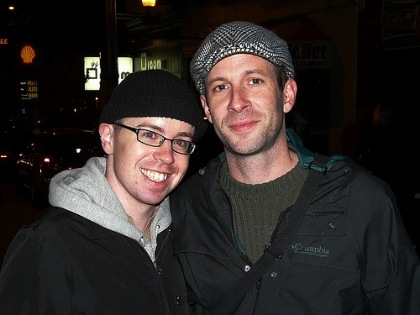
\includegraphics[width=\linewidth]{figures/fail/f01c.jpg}\\[2pt]{\sffamily\footnotesize\raggedright\textit{``a man in a black shirt and a woman in a black shirt and a woman in a white shirt are sitting on a bench''}\\ \textcolor{tfred}{\scriptsize\bfseries INVENTED OBJECT, REPETITION}\par}\end{minipage}\hfill\begin{minipage}[t]{0.315\textwidth}\centering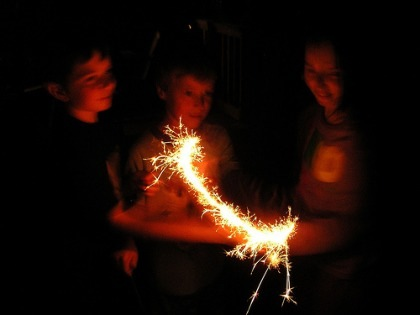
\includegraphics[width=\linewidth]{figures/fail/f02c.jpg}\\[2pt]{\sffamily\footnotesize\raggedright\textit{``a man in a red shirt is standing in front of a crowd''}\\ \textcolor{tfred}{\scriptsize\bfseries WRONG SUBJECT, WRONG COUNT}\par}\end{minipage}\\[8pt]
\begin{minipage}[t]{0.315\textwidth}\centering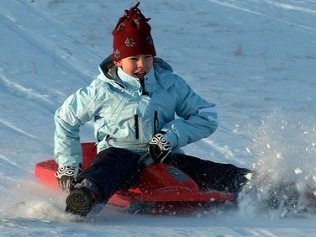
\includegraphics[width=\linewidth]{figures/fail/f03c.jpg}\\[2pt]{\sffamily\footnotesize\raggedright\textit{``a snowboarder in the air''}\\ \textcolor{tfred}{\scriptsize\bfseries WRONG SUBJECT}\par}\end{minipage}\hfill\begin{minipage}[t]{0.315\textwidth}\centering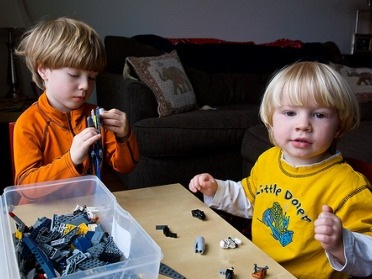
\includegraphics[width=\linewidth]{figures/fail/f04c.jpg}\\[2pt]{\sffamily\footnotesize\raggedright\textit{``a woman in a white shirt and a woman in a white dress are sitting on a couch''}\\ \textcolor{tfred}{\scriptsize\bfseries WRONG SUBJECT, REPETITION}\par}\end{minipage}\hfill\begin{minipage}[t]{0.315\textwidth}\centering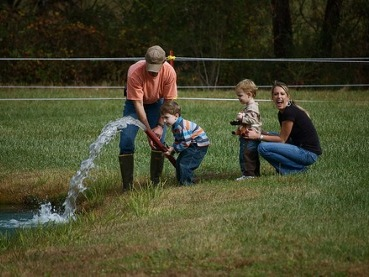
\includegraphics[width=\linewidth]{figures/fail/f05c.jpg}\\[2pt]{\sffamily\footnotesize\raggedright\textit{``a group of children playing soccer''}\\ \textcolor{tfred}{\scriptsize\bfseries INVENTED OBJECT, WRONG COUNT}\par}\end{minipage}\\[8pt]
\begin{minipage}[t]{0.315\textwidth}\centering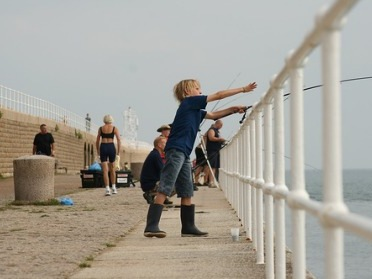
\includegraphics[width=\linewidth]{figures/fail/f06c.jpg}\\[2pt]{\sffamily\footnotesize\raggedright\textit{``a man in a red shirt is standing in front of a \textless unk\textgreater{}''}\\ \textcolor{tfred}{\scriptsize\bfseries WRONG SUBJECT, WRONG COLOUR}\par}\end{minipage}\hfill\begin{minipage}[t]{0.315\textwidth}\centering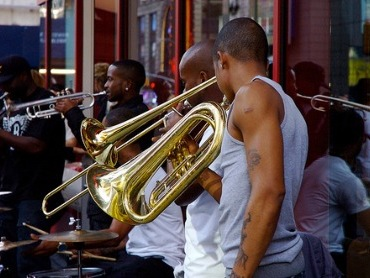
\includegraphics[width=\linewidth]{figures/fail/f07c.jpg}\\[2pt]{\sffamily\footnotesize\raggedright\textit{``a man and a woman are sitting on a bench''}\\ \textcolor{tfred}{\scriptsize\bfseries INVENTED OBJECT, GENERIC}\par}\end{minipage}\hfill\begin{minipage}[t]{0.315\textwidth}\centering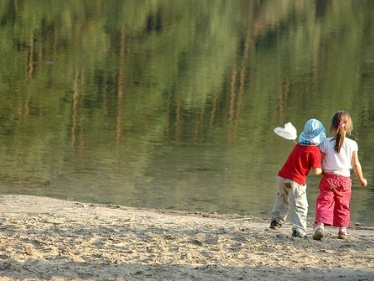
\includegraphics[width=\linewidth]{figures/fail/f08c.jpg}\\[2pt]{\sffamily\footnotesize\raggedright\textit{``a little girl in a pink dress is walking through a field''}\\ \textcolor{tfred}{\scriptsize\bfseries WRONG SUBJECT, INVENTED OBJECT}\par}\end{minipage}\\[8pt]
\begin{minipage}[t]{0.315\textwidth}\centering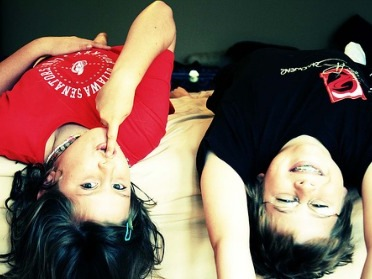
\includegraphics[width=\linewidth]{figures/fail/f09c.jpg}\\[2pt]{\sffamily\footnotesize\raggedright\textit{``a man and a woman pose for a picture''}\\ \textcolor{tfred}{\scriptsize\bfseries NO RULE FIRED}\par}\end{minipage}\hfill\begin{minipage}[t]{0.315\textwidth}\centering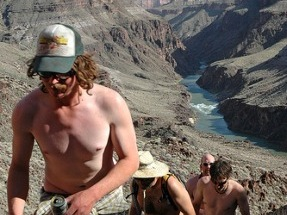
\includegraphics[width=\linewidth]{figures/fail/f10c.jpg}\\[2pt]{\sffamily\footnotesize\raggedright\textit{``a group of people sit on a rock overlooking the ocean''}\\ \textcolor{tfred}{\scriptsize\bfseries WRONG SUBJECT, INVENTED OBJECT, WRONG COUNT}\par}\end{minipage}\hfill\begin{minipage}[t]{0.315\textwidth}\centering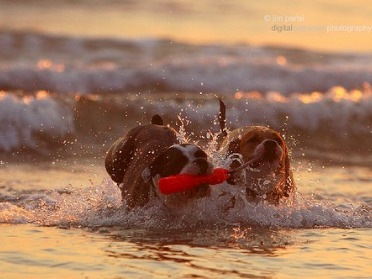
\includegraphics[width=\linewidth]{figures/fail/f11c.jpg}\\[2pt]{\sffamily\footnotesize\raggedright\textit{``a man is riding a surfboard on a beach''}\\ \textcolor{tfred}{\scriptsize\bfseries WRONG SUBJECT, INVENTED OBJECT}\par}\end{minipage}
\caption{The twelve C6 captions with the lowest BLEU-4 score, with the automatic error labels in red. The first one, ``two dogs play in the grass'', is actually correct: it scored low only because the human captions are worded differently, so the automatic labels are not always right.}
\label{fig:fail}
\end{figure}

\textbf{What the encoder sees.} The t-SNE map \cite{vandermaaten2008} of the pooled ResNet50 features (Figure~\ref{fig:tsne}) explains the most common error. Dogs form their own island, so the models rarely confuse them with anything else, but the different kinds of people overlap, so every Part~1 model often names the wrong person.

\textbf{Failure cases.} Figure~\ref{fig:fail} shows that low BLEU does not always mean a wrong caption, and that the automatic error labels are noisy. We therefore quote error rates only as approximate.

\textbf{Photographs outside the dataset.} We also captioned our own photographs through the dashboard. Photos close to Flickr8k (a dog catching a ball, a football match, a person on a beach) received correct and specific captions from the attention models, with heatmaps on the right objects. An empty park bench received ``a man sits on a bench'' from every model: in Flickr8k nearly every bench is occupied, and the models learned that association. The CLIP-encoder model, the best on the test set, added a second person to a photo of a single person on a beach, a reminder that average scores do not guarantee every caption.

%=====================================================================
\section{Discussion}\label{sec:discussion}

\textbf{What matters.} Ranked by effect on CIDEr, with every effect tested: the image encoder (+45\%), attention over image regions (+24\%), then fine-tuning and the recurrent unit (about 5\% each). The hybrid LSTM$\rightarrow$GRU decoder adds nothing over a GRU. For anyone building a captioner under the constraints of this project, effort is best spent on the image representation and on letting the decoder look at regions, not on the recurrent cell.

\textbf{Reproducing the reference paper.} The qualitative claims of \cite{kavitha2025} hold: ResNet50 is a reasonable encoder and beam search helps. The quantitative ones do not transfer. Its accuracy of 0.89 is largely a property of padding, its BLEU-1 of 0.60 comes from 40 images whose selection is not described, and its large gaps between decoders disappear when the decoders are trained identically. None of this implies bad faith; it illustrates how much results depend on details that papers often leave out, and why reporting seeds, full test sets and significance matters.

\textbf{Metrics.} Two metrics in this study can mislead: accuracy that counts padding, and BLEU when caption styles differ. CIDEr, CLIPScore and key-object recall agreed with each other and with our reading of the captions. We recommend reporting at least one reference-based and one reference-free metric.

\textbf{Limitations.} (i) Flickr8k is small; larger datasets (Flickr30k, COCO) would likely narrow the gap to the pretrained models. (ii) Part~2 models were not tuned; the Transformer in particular would benefit from more regularisation. (iii) BLIP was evaluated once and pretrained on far more data, so it is a reference, not a competitor. (iv) Error-type labels are rule-based and approximate. (v) We did not run a human evaluation; CLIPScore is an automatic stand-in. (vi) Paper~1's accuracy could not be reproduced exactly because its protocol is under-specified.

%=====================================================================
\section{Interactive dashboard}\label{sec:dashboard}

To make the results explorable, we built a Streamlit dashboard that runs on a laptop CPU. Its first page captions a photo uploaded or taken with the webcam using C3, A1, A2 and the CLIP-encoder model (optionally BLIP-large), reads the best caption aloud, and lets the user step through the caption word by word to see each word's attention or Grad-CAM map and the model's top five candidate words, together with the beam-search tree for the photo. Further pages present every result table as an interactive chart, the significance tests, the accuracy illusion, a gallery of all 1,000 test images with every model's caption, the hallucination analysis, a clickable t-SNE map and the training curves. A single ResNet50 pass per photo feeds all models.

%=====================================================================
\section{Conclusion and future work}\label{sec:conclusion}

In a controlled, multi-seed study on Flickr8k, the choice of image encoder and the use of attention dominate every other design decision in a CNN--RNN captioner, fine-tuning and the recurrent unit give small real gains, and the hybrid LSTM--GRU decoder brings no benefit over a GRU. The reference paper's headline accuracy is largely an artefact of counting padding. Our best trained model (hybrid decoder on CLIP features, CIDEr 0.582, CLIPScore 0.594) remains clearly below human captions (CLIPScore 0.712) and the pretrained BLIP-large (0.641).

Natural next steps are to combine the two strongest ideas, attention over CLIP's image patches; to train on Flickr30k or COCO; to add a coverage penalty against repetition; and to validate the automatic metrics with a human study.

\section*{Acknowledgements}
This report was prepared for the Deep Learning course (702AI0C008), AY 2026--27, at SVKM's NMIMS Mukesh Patel School of Technology Management \& Engineering.

\section*{Data and code availability}
Flickr8k is available for research use from its original authors \cite{hodosh2013}. All code, configurations, the Colab notebook that reproduces every number, and the dashboard are available from the authors on request.

\bibliographystyle{tfnlm}\small
\bibliography{references}

\clearpage
\appendix
\section{Complete results}

\begin{table}[H]\centering
\tbl{All models on the 1,000 test images. Trained models: mean over three seeds, beam 5. BLIP: one run, beam 3. CLIP-S and RefCLIP-S use CLIP ViT-L/14. CHAIR-s: share of captions naming a non-referenced object.}
{\begin{tabular}{lcccccccc}\toprule
Model & B-1 & B-4 & METEOR & CIDEr & CLIP-S & RefCLIP-S & Key-obj. & CHAIR-s\\\midrule
C1 LSTM & 0.581 & 0.168 & 0.175 & 0.377 & 0.492 & 0.547 & 0.608 & 42.5\%\\
C2 GRU & 0.580 & 0.172 & 0.179 & 0.395 & 0.502 & 0.555 & 0.620 & 36.6\%\\
C3 Hybrid & 0.586 & 0.174 & 0.179 & 0.401 & 0.503 & 0.556 & 0.615 & 40.3\%\\
C4 LSTM ft & 0.585 & 0.172 & 0.179 & 0.392 & 0.497 & 0.551 & 0.616 & 40.2\%\\
C5 GRU ft & 0.590 & 0.179 & 0.183 & 0.414 & 0.508 & 0.562 & 0.630 & 37.9\%\\
C6 Hybrid ft & 0.590 & 0.184 & 0.183 & 0.423 & 0.510 & 0.564 & 0.637 & 38.1\%\\
PP replication & 0.588 & 0.175 & -- & -- & 0.514 & 0.567 & 0.619 & 28.1\%\\
E1 Hybrid + VGG16 & 0.584 & 0.167 & 0.174 & 0.380 & 0.496 & 0.551 & 0.596 & --\\
E2 Hybrid + CLIP & 0.655 & 0.233 & 0.217 & 0.582 & 0.594 & 0.646 & 0.790 & --\\
A1 LSTM + attention & 0.629 & 0.221 & 0.203 & 0.524 & 0.549 & 0.598 & 0.657 & 26.2\%\\
A2 Transformer & 0.617 & 0.210 & 0.199 & 0.500 & 0.551 & 0.603 & 0.641 & 25.2\%\\
B1 BLIP-base & 0.648 & 0.263 & 0.212 & 0.665 & 0.612 & 0.667 & 0.716 & 11.3\%\\
B2 BLIP-large & 0.626 & 0.206 & 0.259 & 0.693 & 0.641 & 0.695 & 0.841 & 26.0\%\\\midrule
Human reference & -- & -- & -- & -- & 0.712 & 0.744 & -- & --\\\bottomrule
\end{tabular}}
\tabnote{``--'' = not computed for that model. PP: paper-protocol replication (single seed).}
\label{tab:all}
\end{table}

\begin{table}[H]\centering
\tbl{Paired bootstrap tests (CIDEr and CLIPScore, Holm-corrected).}
{\begin{tabular}{lcccc}\toprule
Comparison (A vs B) & $\Delta$CIDEr & 95\% CI & $p$ & $p$ (CLIP-S)\\\midrule
GRU vs LSTM (frozen) & +0.018 & [+0.003, +0.033] & 0.049 & 0.001\\
Hybrid vs LSTM (frozen) & +0.024 & [+0.009, +0.039] & 0.006 & 0.001\\
Hybrid vs GRU (frozen) & +0.006 & [$-$0.009, +0.021] & 0.400 & 0.810\\
Fine-tuning, LSTM & +0.015 & [+0.005, +0.026] & 0.012 & 0.013\\
Fine-tuning, GRU & +0.019 & [+0.008, +0.031] & 0.011 & 0.001\\
Fine-tuning, hybrid & +0.022 & [+0.009, +0.035] & 0.008 & 0.001\\
ResNet50 vs VGG16 & +0.021 & [+0.003, +0.039] & 0.049 & 0.016\\
CLIP vs ResNet50 & +0.180 & [+0.155, +0.206] & 0.001 & 0.001\\
A1 attention vs C6 & +0.100 & [+0.078, +0.123] & 0.001 & 0.001\\
A2 Transformer vs A1 & $-$0.023 & [$-$0.040, $-$0.006] & 0.028 & 0.506\\
CLIP encoder vs A1 & +0.058 & [+0.032, +0.085] & 0.001 & 0.001\\\bottomrule
\end{tabular}}
\tabnote{$p=0.001$ is the smallest value 10,000 resamples and the Holm correction can produce here.}
\end{table}

\end{document}
